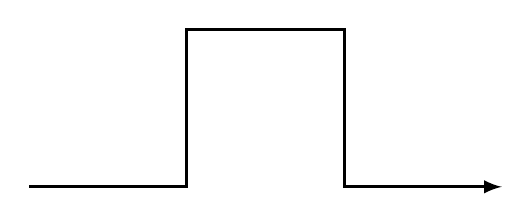
\begin{tikzpicture}
    \coordinate (M1) at (-1,0); 
    \coordinate (M2) at (-1,2); 
    \coordinate (M3) at (1,2);
    \coordinate (M4) at (1,0); 
    \draw[very thick, -{latex}] (-3,0) -- (M1) -- (M2) -- (M3) -- (M4) -- (3,0);
    \mirror[angle=-45] at (M1);
    \mirror[angle=135, color=optikzred, shift=0.5] at (M2);
    \mirror[angle=45, color=optikzred, shift=-0.5] at (M3);
    \mirror[angle=225] at (1,0);
\end{tikzpicture}